\tikzstyle{input_neuron}=[circle,draw=red!50,fill=orange!10,thick,minimum size=.2mm]
\tikzstyle{hidden_neuron}=[circle,draw=blue!50,fill=blue!10,thick,minimum size=1mm]
\tikzstyle{output_neuron}=[circle,draw=green!50,fill=green!20,thick,minimum size=1mm]
\tikzstyle{input}=[circle,draw=black!50,fill=black!20,thick,minimum size=.2mm]
\begin{tikzpicture}

	\node [input_neuron] (neuron0) at (7,3)  {$\sigma$} ;
	\node (input0) at (7,1.5)  {$x=h_{0}$};
	
	\node [hidden_neuron] (neuron1) at (7,4.5)  {$\sigma$};
	\node [output_neuron] (neuron2) at (7,6)  {$\sigma$} ;
	
	\node (output0)  at (7,7.5) {$y$};
	
	\draw [->] (input0) -- (neuron0);
	\draw [->] (neuron0) -- (neuron1);
	\draw [->] (neuron1) -- (neuron2);
	\draw [->] (neuron2) -- (output0);
	\only<16->{\draw[green,dashed] (6.5,6) -- (7.5,6);}
	\only<11->{\draw[blue,dashed] (6.5,4.5) -- (7.5,4.5);}
	\only<6->{\draw[red,dashed] (6.5,3) -- (7.5,3);}
	
	\node (formula) at (6.7,2.25) {$w_{1}$};
	\node (formula) at (6.7,3.75) {$w_{2}$};
	\node (formula) at (6.7,5.) {$w_{3}$};
	
	\only<7->{\node (formula) at (7.3,2.6) {$a_{1}$};}
	\only<9->{\node (formula) at (7.3,3.45) {$h_{1}$};}
	\only<12->{\node (formula) at (7.3,4.1) {$a_{2}$};}
	\only<14->{\node (formula) at (7.3,4.95) {$h_{2}$};}
	\only<16->{\node (formula) at (7.3,5.6) {$a_{3}$};}
	\only<16->{\node (formula) at (7.3,6.45) {$h_{3}$};}
	
\end{tikzpicture}